\documentclass[12pt, titlepage]{article}

\usepackage{booktabs}
\usepackage{tabularx}
\usepackage{hyperref}
\hypersetup{ colorlinks, citecolor=blue, filecolor=black, linkcolor=red,
    urlcolor=blue }
\usepackage[round]{natbib}
\usepackage{graphicx}

%% Comments

\usepackage{color}

\newif\ifcomments\commentstrue %displays comments
%\newif\ifcomments\commentsfalse %so that comments do not display

\ifcomments
\newcommand{\authornote}[3]{\textcolor{#1}{[#3 ---#2]}}
\newcommand{\todo}[1]{\textcolor{red}{[TODO: #1]}}
\else
\newcommand{\authornote}[3]{}
\newcommand{\todo}[1]{}
\fi

\newcommand{\wss}[1]{\authornote{blue}{SS}{#1}} 
\newcommand{\plt}[1]{\authornote{magenta}{TPLT}{#1}} %For explanation of the template
\newcommand{\an}[1]{\authornote{cyan}{Author}{#1}}

%% Common Parts

\newcommand{\progname}{ProgName} % PUT YOUR PROGRAM NAME HERE
\newcommand{\authname}{Team \#, Team Name
\\ Student 1 name
\\ Student 2 name
\\ Student 3 name
\\ Student 4 name} % AUTHOR NAMES                  

\usepackage{hyperref}
    \hypersetup{colorlinks=true, linkcolor=blue, citecolor=blue, filecolor=blue,
                urlcolor=blue, unicode=false}
    \urlstyle{same}
                                


\usepackage{enumitem,amssymb}
\newlist{todolist}{itemize}{2}
\setlist[todolist]{label=$\square$}

\newcommand{\tcref}[1]{TC\ref{#1}} \newcounter{testcasenum}
\newcommand{\tthetestcasenum}{TM\thetestcasenum}

\begin{document}

\title{System Verification and Validation Plan for \progname{}} 
\author{\authname}
\date{\today}
	
\maketitle

\pagenumbering{roman}

\section*{Revision History}

\begin{tabularx}{\textwidth}{p{3cm}p{2cm}X} \toprule {\bf Date} & {\bf Version}
& {\bf Notes}\\
\midrule
Feb 21, 2025 & 1.0 & Creation\\
\bottomrule
\end{tabularx}

~\\
\wss{The intention of the VnV plan is to increase confidence in the software.
However, this does not mean listing every verification and validation technique
that has ever been devised.  The VnV plan should also be a \textbf{feasible}
plan. Execution of the plan should be possible with the time and team available.
If the full plan cannot be completed during the time available, it can either be
modified to ``fake it'', or a better solution is to add a section describing
what work has been completed and what work is still planned for the future.}

\wss{The VnV plan is typically started after the requirements stage, but before
the design stage.  This means that the sections related to unit testing cannot
initially be completed.  The sections will be filled in after the design stage
is complete.  the final version of the VnV plan should have all sections filled
in.}

\newpage

\tableofcontents

\listoftables
\wss{Remove this section if it isn't needed}

\listoffigures
\wss{Remove this section if it isn't needed}

\newpage

\section{Symbols, Abbreviations, and Acronyms}

The definitions of symbols, abbreviations, and acronyms used in this document
are consistent with those provided in SRS\citep{SRS}.

\newpage

\pagenumbering{arabic}

This document outlines the Verification and Validation Plan (VnV) for \progname,
structured into four main sections.  General Information includes the summary,
objectives, challenge level and extras relevant to the VnV process.  Plan
details the verification strategy for the SRS, Design, VnV, and Implementation
phases, along with the use of automated testing and verification tools, as well
as software validation plan. System Tests verify both functional and
nonfunctional requirements at the system level, ensuring the overall system
meets its intended behavior.  Unit Test Description covers validating individual
modules against both functional and nonfunctional requirements.  This plan
ensures a comprehensive and systematic approach to verifying and validating the
system before deployment.

\section{General Information}

This section will provide the project summary and objectives for this document.

\subsection{Summary}

This project focuses on reimplementing the Pan-Tompkins algorithm for R-wave
detection in ECG signal processing.  This implementation will automatically
derive all filter parameters based on requirements without relying on external
libraries.

\subsection{Objectives}

The objectives of this VnV plan include:

\begin{itemize}
  \item Build confidence in the software correctness.
  \item Test robustness against noisy ECG signals.
\end{itemize}

\noindent The objectives of this VnV plan do not include:

\begin{itemize}
  \item User experience testing for a graphical interface or integration into
  medical workflow systems.
  \item Clinical trials.
\end{itemize}

\subsection{Challenge Level and Extras}

This is a problem with a general-level challenge. Doxygen will be widely used to
generate the API documentation.

\subsection{Relevant Documentation}

In the Verification and Validation Plan, we reference the Software Requirements
Specification (SRS) \citep{SRS} as the primary document. The SRS outlines the
system’s requirements, forming the foundation for all verification activities.
It ensures that the VnV process is aligned with the specified functional and
nonfunctional requirements.

\section{Plan}

\wss{Introduce this section.  You can provide a roadmap of the sections to
  come.}

% \subsection{Verification and Validation Team}

% \wss{Your teammates.  Maybe your supervisor.  You should do more than list
%   names.  You should say what each person's role is for the project's
%   verification.  A table is a good way to summarize this information.}

\subsection{SRS Verification Plan}

The SRS document \citep{SRS} will be reviewed by a domain expert.  The content
of the review is based on the following checklist:

\begin{todolist}
  \item Completeness: Included GS, A, GD, DD, TM, IM, etc.
  \item Formatting: The document has a clear, logical structure, and properly
  organized.
  \item Verifiability: Each requirement is testable with a clear pass/fail
  standard.
  \item Traceability: Each requirement is linked to an IM
\end{todolist}

\subsection{Design Verification Plan}

The Design Verification Plan will be reviewed by a domain expert.  The content
of the review is based on the following checklist:

\begin{todolist}
  \item Low module coupling: modules can be reused anywhere and do not affect
  others.
  \item Good Hierarchy: make sure the hierarchy is clear and easy to maintain.
\end{todolist}

\subsection{Verification and Validation Plan Verification Plan}

The Verification and Validation Plan (This document itself) will be reviewed by
a domain expert.  The content of the review is based on the following checklist:

\begin{todolist}
  \item Completeness : VnV plan includes all necessary sections.
  \item Formatting: The document has a clear, logical structure, and properly
  organized.
  \item Appropriateness: Confirm that the methods and tools proposed in the VnV
  plan are appropriate for the project.
  \item Coverage: Make sure the VnV plan covers all the requirements.
\end{todolist}

\subsection{Implementation Verification Plan}

\wss{You should at least point to the tests listed in this document and the unit
  testing plan.}

\wss{In this section you would also give any details of any plans for static
  verification of the implementation.  Potential techniques include code
  walkthroughs, code inspection, static analyzers, etc.}

\wss{The final class presentation in CAS 741 could be used as a code
walkthrough.  There is also a possibility of using the final presentation (in
CAS741) for a partial usability survey.}

\subsection{Automated Testing and Verification Tools}

\begin{itemize}
  \item Static code checker: cpplint - A tool that enforces Google's C++ style
  guide by checking for common coding style violations.
  \item Unit test: gTest - A C++ testing framework that provides a rich set of
  assertions and test case management.
  \item Test coverage: gcov - A test coverage analysis tool for C++ that works with GCC.
  \item Local code quality control: git pre-commit - A framework that runs
  checks before committing code, helping to enforce coding standards and catch
  issues early.
  \item Continuous integration: GitHub Actions - An automation tool that enables
  CI/CD workflows, allowing code to be built, tested, and deployed
  automatically.
\end{itemize}

\subsection{Software Validation Plan}

\wss{If there is any external data that can be used for validation, you should
  point to it here.  If there are no plans for validation, you should state that
  here.}

\wss{You might want to use review sessions with the stakeholder to check that
the requirements document captures the right requirements.  Maybe task based
inspection?}

\wss{For those capstone teams with an external supervisor, the Rev 0 demo should
be used as an opportunity to validate the requirements.  You should plan on
demonstrating your project to your supervisor shortly after the scheduled Rev 0
demo.  
The feedback from your supervisor will be very useful for improving your
project.}

\wss{For teams without an external supervisor, user testing can serve the same
purpose as a Rev 0 demo for the supervisor.}

\wss{This section might reference back to the SRS verification section.}

\section{System Tests}

\wss{There should be text between all headings, even if it is just a roadmap of
the contents of the subsections.}

\subsection{Tests for Functional Requirements}

\wss{Subsets of the tests may be in related, so this section is divided into
  different areas.  If there are no identifiable subsets for the tests, this
  level of document structure can be removed.}

\wss{Include a blurb here to explain why the subsections below cover the
  requirements.  References to the SRS would be good here.}

\refstepcounter{testcasenum} \label{TC_IIR_FIR}
\subsubsection{TC\thetestcasenum : Basic IIR and FIR Filters}

\wss{It would be nice to have a blurb here to explain why the subsections below
  cover the requirements.  References to the SRS would be good here.  If a
  section covers tests for input constraints, you should reference the data
  constraints table in the SRS.}
		
%\paragraph{Title for Test}

\begin{enumerate}

\item{FIR Filter with Random Coefficients\\}

Control: Automatic
					
Initial State: No prior state is required; the test starts with randomly
generated filter coefficients.
					
Input:
\begin{itemize}
  \item FIR filter coefficients generated using scipy.signal.firwin(10, 0.3).
  \item A sinusoidal wave with added Gaussian noise, generated using np.sin(2 *
  np.pi * 0.05 * np.arange(1000)) + np.random.normal(0, 1, 1000).
\end{itemize}

Output:
\begin{itemize}
  \item The filtered signal produced by the implemented FIR filter should
  closely match the filtered signal from scipy.signal.lfilter.
  \item The RMSE between the two outputs should be below $1e-5$.
\end{itemize}

Test Case Derivation: The test ensures that a basic FIR filter implementation
behaves consistently with pseudo-oracle scipy.signal.
					
How test will be performed: 
\begin{enumerate}
  \item Generate FIR filter coefficients.
  \item Generate an input signal as a sinusoidal wave with Gaussian noise.
  \item Apply the FIR filter implementation.
  \item Apply scipy.signal.lfilter with the same coefficients.
  \item Compute the RMSE between outputs.
  \item Assert that the RMSE is below $1e-5$.
\end{enumerate}
					
\item{IIR Filter with Random Coefficients\\}

Control: Automatic
					
Initial State: No prior state is required; the test starts with randomly
generated filter coefficients.
					
Input:
\begin{itemize}
  \item IIR filter coefficients generated using scipy.signal.butter(3, 0.3,
  btype='low', output='ba').
  \item A sinusoidal wave with added Gaussian noise, generated using np.sin(2 *
  np.pi * 0.05 * np.arange(1000)) + np.random.normal(0, 1, 1000).
\end{itemize}

Output:
\begin{itemize}
  \item The filtered signal produced by the implemented IIR filter should
  closely match the filtered signal from scipy.signal.lfilter.
  \item The RMSE between the two outputs should be below $1e-5$.
\end{itemize}

The test ensures that a basic IIR filter implementation behaves consistently
with scipy.signal.

How test will be performed: 
\begin{enumerate}
  \item Generate IIR filter coefficients.
  \item Generate an input signal as a sinusoidal wave with Gaussian noise.
  \item Apply the IIR filter implementation.
  \item Apply scipy.signal.lfilter with the same coefficients.
  \item Compute the RMSE between outputs.
  \item Assert that the RMSE is below $1e-5$.
\end{enumerate}

\end{enumerate}

\refstepcounter{testcasenum} \label{TC_BUT_CHEB}
\subsubsection{TC\thetestcasenum : Butterworth and Chebyshev Filters}

\begin{enumerate}

  \item{Butterworth Low-Pass Filter\\}
  
  Control: Automatic
            
  Initial State: No prior state is required; the test starts with selected
  filter parameters.
            
  Input:
  \begin{itemize}
    \item Cutoff frequency: $f_c=0.3$
    \item Filter order $N=4$
    \item Filter coefficients generated using scipy.signal.butter(4, 0.3,
    btype='low', output='ba').
  \end{itemize}
  
  Output:
  \begin{itemize}
    \item The computed filter coefficients should match those generated by
    scipy.signal.butter.
    \item The RMSE between the two outputs should be below $1e-5$.
  \end{itemize}
  
  Test Case Derivation: The test ensures that a Butterworth filter
  implementation behaves consistently with pseudo-oracle scipy.signal.
            
  How test will be performed: 
  \begin{enumerate}
    \item Generate Butterworth filter coefficients by scipy.signal.butter.
    \item Generate Butterworth filter coefficients by implementation.
    \item Compute the RMSE between the implemented and scipy.signal
    coefficients.
    \item Assert that the RMSE is below 1e-5.
  \end{enumerate}
            
  \item{Chebyshev Type I Low-Pass Filter\\}
  
  Control: Automatic
            
  Initial State: No prior state is required; the test starts with selected
  filter parameters.
            
  Input:
  \begin{itemize}
    \item Cutoff frequency: $f_c=0.3$
    \item Filter order $N=4$
    \item Passband ripple: $0.5 dB$
    \item Filter coefficients generated using scipy.signal.cheby1(4, 0.5, 0.3,
    btype='low', output='ba').
  \end{itemize}
  
  Output:
  \begin{itemize}
    \item The filtered signal produced by the implemented Chebyshev filter
    should closely match the filtered signal from scipy.signal.lfilter.
    \item The RMSE between the two outputs should be below $1e-5$.
  \end{itemize}
  
  The test ensures that a Chebyshev implementation behaves consistently with
  scipy.signal.
  
  How test will be performed: 
  \begin{enumerate}
    \item Generate Chebyshev filter coefficients by scipy.signal.cheby1.
    \item Generate Chebyshev filter coefficients by implementation.
    \item Compute the RMSE between the implemented and scipy.signal
    coefficients.
    \item Assert that the RMSE is below 1e-5.
  \end{enumerate}
  
\end{enumerate}

\refstepcounter{testcasenum} \label{TC_SQUARING}
\subsubsection{TC\thetestcasenum : Squaring function}

\begin{enumerate}

  \item{Sequence input test\\}
  
  Control: Automatic
            
  Initial State: No prior state is required.
            
  Input:
  \begin{itemize}
    \item $[1.2, -2.1, -1.0, 2.0, 3.0]$
  \end{itemize}
  
  Output:
  \begin{itemize}
    \item $[1.44, 4.41, 1.0, 4.0, 9.0]$
  \end{itemize}
  
  Test Case Derivation: The purpose of this test case is to verify that the
  squaring function correctly squares each value in the input list, regardless
  of whether the numbers are positive or negative. The function should return
  the squared value of each element from the input list.

  The input given here is just an example.  In practice, the input will be a
  large amount of data randomly generated by the program for testing.
            
  How test will be performed: 
  \begin{enumerate}
    \item The input list will be provided to the squaring function.
    \item The function will process each element in the list and square it.
    \item The output will be compared against the expected result.
    \item There is a global floating point comparison threshold $\epsilon$ to
    determine whether floating point numbers are equal.
  \end{enumerate}

\end{enumerate}

\refstepcounter{testcasenum} \label{TC_THRESHOLDING}
\subsubsection{TC\thetestcasenum : Thresholding function}

\begin{enumerate}

  \item{Sequence input test\\}
  
  Control: Automatic
            
  Initial State: No prior state is required.
            
  Input:
  \begin{itemize}
    \item input sequence: $[1.44, 4.2, 1.0, 4.0, 9.0]$
    \item dynamic threshold: $[3.7, 3.8, 3.9, 3.6, 3.2]$
  \end{itemize}
  
  Output:
  \begin{itemize}
    \item $[0, 4.2, 0, 4.0, 9.0]$
  \end{itemize}
  
  Test Case Derivation: This test case aims to verify that the thresholding
  function correctly applies dynamic thresholds to each element in the input
  sequence.  For each element in the sequence, if the value is greater than the
  corresponding threshold, it should remain unchanged; otherwise, it should be
  replaced with $0$.

  The input given here is just an example.  In practice, the input will be a
  large amount of data randomly generated by the program for testing.
            
  How test will be performed: 
  \begin{enumerate}
    \item The input sequence and dynamic thresholds will be provided to the
    thresholding function.
    \item The function will process each element in the list.
    \item The output will be compared against the expected result.
    \item There is a global floating point comparison threshold $\epsilon$ to
    determine whether floating point numbers are equal.
  \end{enumerate}

\end{enumerate}

\refstepcounter{testcasenum} \label{TC_RMSE}
\subsubsection{TC\thetestcasenum : RMSE calculating function}

\begin{enumerate}

  \item{Sequence input test\\}
  
  Control: Automatic
            
  Initial State: No prior state is required.
            
  Input:
  \begin{itemize}
    \item input sequence 1: $[100, 200, 300, 400, 500]$
    \item input sequence 2: $[99, 203, 300, 398, 501]$
  \end{itemize}
  
  Output:
  \begin{itemize}
    \item $RMSE = 1.732$
  \end{itemize}
  
  Test Case Derivation: This test case verifies that the RMSE function correctly
  calculates the root mean squared error between two input sequences.  The RMSE
  is calculated as the square root of the mean of the squared differences
  between corresponding elements of the two sequences.

  The input given here is just an example.  In practice, the input will be a
  large amount of data randomly generated by the program for testing.
            
  How test will be performed: 
  \begin{enumerate}
    \item Two input sequences will be provided to the thresholding function.
    \item The function will process two input sequences and return the RMSE.
    \item The output will be compared against the expected result.
    \item There is a global floating point comparison threshold $\epsilon$ to
    determine whether floating point numbers are equal.
  \end{enumerate}

\end{enumerate}

\refstepcounter{testcasenum} \label{TC_ALG}
\subsubsection{TC\thetestcasenum : R-wave position calculating}

\begin{enumerate}

  \item{MIT-BIH Database test\\}
  
  Control: Automatic
            
  Initial State: No prior state is required.
            
  Input:
  \begin{itemize}
    \item sampling frequency $f_s=360$ Hz
    \item MIT-BIH data from
    \url{https://www.physionet.org/content/mitdb/1.0.0/}, as shown in figure
    \ref{Fig_wave}. This is a curve consisting of discrete sample points and
    contains the annotated points from cardiologists.  The blue vertical lines
    in the figure \ref{Fig_wave} are annotated points.
  \end{itemize}

  \begin{figure}[h!]
    \begin{center}
      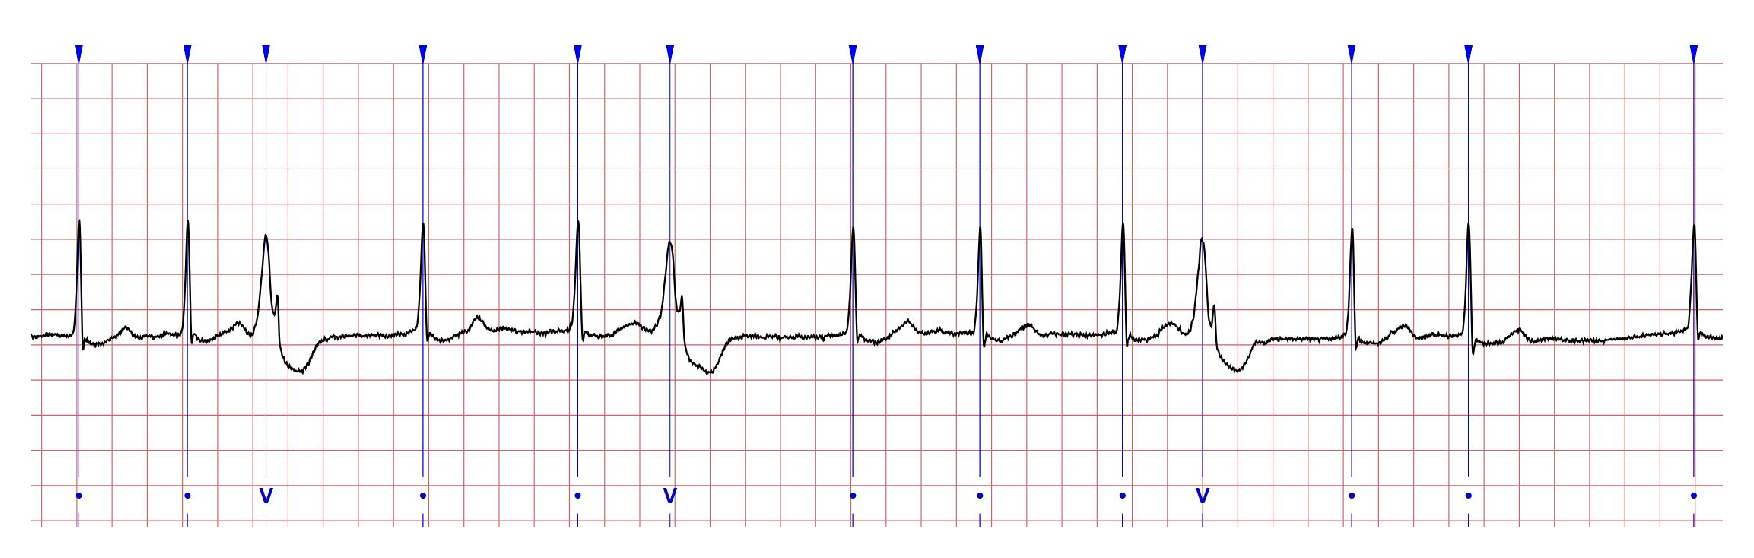
\includegraphics[width=1.1\textwidth]{wave}
      \caption{input wave}
      \label{Fig_wave} 
    \end{center}
  \end{figure}
  
  Output:
  \begin{itemize}
    \item The index of annotated points from cardiologists as shown in figure
    \ref{Fig_wave}.
    \item The RMSE between calculated and annotated R-wave index.
  \end{itemize}
  
  Test Case Derivation: The test will evaluate the accuracy of the R-wave
  detection function by comparing the detected R-wave index to the annotated
  index, with the RMSE between the two sets of index expected to be below $3.0$.
            
  How test will be performed: 
  \begin{enumerate}
    \item The input $f_s$ and wave data will be provided to the calculating
    function.
    \item The annotated data will be provided to the calculating function.
    \item The function will process the original wave data and calculate the
    R-wave index.
    \item The function will return the RMSE.
    \item The correctness of this function is evaluated by the output RMSE,
    assert that the RMSE is below $3.0$.
  \end{enumerate}

\end{enumerate}

\subsection{Tests for Nonfunctional Requirements}

\refstepcounter{testcasenum} \label{TC_USABILITY}
\subsubsection{TC\thetestcasenum : Usability}

\begin{enumerate}

  \item{Verify Doxygen generates a structured and readable API documentation \\}

  Type: Non-Functional, Dynamic, Manual

  Initial State: The software documentation is written in a format supported by
  Doxygen.

  Input/Condition: Run Doxygen on the project’s documentation source files.

  Output/Result: A structured and readable API documentation is generated in the
  expected format (e.g., HTML, PDF).

  How test will be performed:
  \begin{enumerate}
    \item Execute Doxygen with the configured settings.
    \item Inspect the generated documentation for completeness and readability.
    \item Verify that all sections (e.g., class descriptions, function
    documentation) are properly formatted.
    \item Conduct a peer review to assess usability.
  \end{enumerate}
\end{enumerate}

\refstepcounter{testcasenum} \label{TC_MAINTAINABILITY}
\subsubsection{TC\thetestcasenum : Maintainability}

\begin{enumerate}

  \item{Ensure high test coverage \\}

  Type: Non-Functional, Dynamic, Automatic

  Initial State: The software project contains multiple modules.

  Input/Condition: Run a test coverage analysis tool (gcov).

  Output/Result: A report showing the percentage of code covered by tests.

  How test will be performed:
  \begin{enumerate}
    \item Execute the test suite with coverage tracking enabled.
    \item Generate a test coverage report.
    \item Verify that all modules have test coverage above a predefined
    threshold.
    \item If any module lacks coverage, update tests accordingly.
  \end{enumerate}
\end{enumerate}

\refstepcounter{testcasenum} \label{TC_PORTABILITY}
\subsubsection{TC\thetestcasenum : Portability}

\begin{enumerate}

  \item{Confirm the software builds and runs correctly on multi-platform \\}

  Type: Non-Functional, Dynamic, Manual

  Initial State: The source code is available and ready for compilation.

  Input/Condition: Attempt to build and run the software on both Linux and
  Windows environments.

  Output/Result: The software compiles successfully and functions correctly on
  both platforms.

  How test will be performed:
  \begin{enumerate}
    \item Set up test environments for Linux and Windows.
    \item Compile the software on both platforms.
    \item Run key functionalities and verify expected behavior.
    \item Identify and document any platform-specific issues.
  \end{enumerate}
\end{enumerate}

\refstepcounter{testcasenum} \label{TC_REUSABILITY}
\subsubsection{TC\thetestcasenum : Reusability}

\begin{enumerate}

  \item{Check if the code is modular and reusable in different contexts \\}

  Type: Non-Functional, Static, Manual

  Initial State: The software project contains multiple modules.

  Input/Condition: Review code structure and check module usage.

  Output/Result: A checklist ensures that modules are used in different
  contexts.

  How test will be performed:
  \begin{enumerate}
    \item Inspect code structure for clear separation of concerns.
    \item Identify modules that are used in different parts of the software.
    \item Complete a module reuse checklist, and suggest improvements for better
    modularity.
  \end{enumerate}
\end{enumerate}

\subsection{Traceability Between Test Cases and Requirements}

\wss{Provide a table that shows which test cases are supporting which
  requirements.}

\section{Unit Test Description}

\wss{This section should not be filled in until after the MIS (detailed design
  document) has been completed.}

\wss{Reference your MIS (detailed design document) and explain your overall
philosophy for test case selection.}  

\wss{To save space and time, it may be an option to provide less detail in this
section.  
For the unit tests you can potentially layout your testing strategy here.  That
is, you can explain how tests will be selected for each module.  For instance,
your test building approach could be test cases for each access program,
including one test for normal behaviour and as many tests as needed for edge
cases.  Rather than create the details of the input and output here, you could
point to the unit testing code.  For this to work, you code needs to be
well-documented, with meaningful names for all of the tests.}

\subsection{Unit Testing Scope}

\wss{What modules are outside of the scope.  If there are modules that are
  developed by someone else, then you would say here if you aren't planning on
  verifying them.  There may also be modules that are part of your software, but
  have a lower priority for verification than others.  If this is the case,
  explain your rationale for the ranking of module importance.}

\subsection{Tests for Functional Requirements}

\wss{Most of the verification will be through automated unit testing.  If
  appropriate specific modules can be verified by a non-testing based technique.
  That can also be documented in this section.}

\subsubsection{Module 1}

\wss{Include a blurb here to explain why the subsections below cover the module.
  References to the MIS would be good.  You will want tests from a black box
  perspective and from a white box perspective.  Explain to the reader how the
  tests were selected.}

\begin{enumerate}

\item{test-id1\\}

Type: \wss{Functional, Dynamic, Manual, Automatic, Static etc. Most will be
  automatic}
					
Initial State: 
					
Input: 
					
Output: \wss{The expected result for the given inputs}

Test Case Derivation: \wss{Justify the expected value given in the Output field}

How test will be performed: 
					
\item{test-id2\\}

Type: \wss{Functional, Dynamic, Manual, Automatic, Static etc. Most will be
  automatic}
					
Initial State: 
					
Input: 
					
Output: \wss{The expected result for the given inputs}

Test Case Derivation: \wss{Justify the expected value given in the Output field}

How test will be performed: 

\item{...\\}
    
\end{enumerate}

\subsubsection{Module 2}

...

\subsection{Tests for Nonfunctional Requirements}

\wss{If there is a module that needs to be independently assessed for
  performance, those test cases can go here.  In some projects, planning for
  nonfunctional tests of units will not be that relevant.}

\wss{These tests may involve collecting performance data from previously
  mentioned functional tests.}

\subsubsection{Module ?}
		
\begin{enumerate}

\item{test-id1\\}

Type: \wss{Functional, Dynamic, Manual, Automatic, Static etc. Most will be
  automatic}
					
Initial State: 
					
Input/Condition: 
					
Output/Result: 
					
How test will be performed: 
					
\item{test-id2\\}

Type: Functional, Dynamic, Manual, Static etc.
					
Initial State: 
					
Input: 
					
Output: 
					
How test will be performed: 

\end{enumerate}

\subsubsection{Module ?}

...

\subsection{Traceability Between Test Cases and Modules}

\wss{Provide evidence that all of the modules have been considered.}
				
\bibliographystyle{plainnat}

\bibliography{../../refs/References}

\newpage

\section{Appendix}

This is where you can place additional information.

\subsection{Symbolic Parameters}

The definition of the test cases will call for SYMBOLIC\_CONSTANTS.  Their
values are defined in this section for easy maintenance.

\subsection{Usability Survey Questions?}

\wss{This is a section that would be appropriate for some projects.}

\newpage{}
\section*{Appendix --- Reflection}

\wss{This section is not required for CAS 741}

The information in this section will be used to evaluate the team members on the
graduate attribute of Lifelong Learning.

The purpose of reflection questions is to give you a chance to assess your own
learning and that of your group as a whole, and to find ways to improve in the
future. Reflection is an important part of the learning process.  Reflection is
also an essential component of a successful software development process.  

Reflections are most interesting and useful when they're honest, even if the
stories they tell are imperfect. You will be marked based on your depth of
thought and analysis, and not based on the content of the reflections
themselves. Thus, for full marks we encourage you to answer openly and honestly
and to avoid simply writing ``what you think the evaluator wants to hear.''

Please answer the following questions.  Some questions can be answered on the
team level, but where appropriate, each team member should write their own
response:


\begin{enumerate}
  \item What went well while writing this deliverable? 
  \item What pain points did you experience during this deliverable, and how did
    you resolve them?
  \item What knowledge and skills will the team collectively need to acquire to
  successfully complete the verification and validation of your project?
  Examples of possible knowledge and skills include dynamic testing knowledge,
  static testing knowledge, specific tool usage, Valgrind etc.  You should look
  to identify at least one item for each team member.
  \item For each of the knowledge areas and skills identified in the previous
  question, what are at least two approaches to acquiring the knowledge or
  mastering the skill?  Of the identified approaches, which will each team
  member pursue, and why did they make this choice?
\end{enumerate}

\end{document}